%----------------------------------------------------------------------------------------
%	PART
%----------------------------------------------------------------------------------------

\part{기말고사 범위}

%----------------------------------------------------------------------------------------
%	CHAPTER 4
%----------------------------------------------------------------------------------------


\chapter{전자기파}
\section{맥스웰 방정식}
지금까지 우리가 살펴본 전자기학의 방정식들을 모두 모아 보자면 다음과 같다.
\begin{align}
\oint \vec{E}\cdot d\vec{a}&=\frac{q_{in}}{\epsilon_0}\\
\oint \vec{B}\cdot d\vec{a}&=0\\
\oint \vec{E}\cdot d\vec{l}&=-\frac{d\Phi_B}{dt}\\
\oint \vec{B}\cdot d\vec{l}&=\mu_0 i_{enc}\label{eqn:ampere}
\end{align}
이 중 식 \ref{eqn:ampere}은 맥스웰에 의해 다음과 같이 수정되었다.
\begin{equation}
\oint \vec{B}\cdot d\vec{l}=\mu_0\epsilon_0 \frac{d\Phi_E}{dt}+\mu_0 i_{enc}
\end{equation}
이를 맥스웰-앙페르 법칙이라고 한다. 여기서 새로 추가된 항 $\mu_0\epsilon_0 \frac{d\Phi_E}{dt}$는 패러데이 법칙과 유사하지만 단위를 맞추기 위한 $\mu_0\epsilon_0$가 추가되었고 방향이 반대이고, 즉, 유도 자기장의 방향은 오른손 법칙이 결정하는 것의 반대 방향이다. \\
식에서 보면 $\epsilon_0 \frac{d\Phi_E}{dt}$의 단위가 전류와 같다는 것을 알 수 있다. 이를 변위 전류(displacement current)라고 하며, $i_d$로 쓴다. 따라서 맥스웰-앙페르 법칙은 
\begin{equation}
\oint \vec{B}\cdot d\vec{l}=\mu_0(i_{enc}+i_d)
\end{equation}
로 쓸 수 있다. 
\begin{example}[평행판 축전기의 충전]\label{dispcur}
반지름이 $R$인 원통형의 평행판 축전기에 $i$의 전류가 흐르면서 충전되고 있다. 이때 변위전류의 크기를 구하고 축전기의 축에서 반지름 방향으로 $d>R$만큼 떨어진 지점에서의 자기장을 구하여라.
\end{example}
\begin{figure}[h]
\centering\includegraphics[scale=0.4]{Pictures/dispcur.PNG}
\caption{Example \ref{dispcur}}
\label{fig:dispcur}
%\addcontentsline{toc}{figure}{Figure \ref{fig:placeholder}} % Uncomment to add the figure to the table of contents
\end{figure}
$\dfrac{dq}{dt}=i$이고 전기장은 $E=\dfrac{\sigma}{\epsilon_0}=\dfrac{q}{\epsilon_0\pi R^2}$이다. 따라서  
\begin{equation}
i_d=\epsilon_0\frac{d\Phi_E}{dt}=i
\end{equation}
이다. $\oint \vec{B}\cdot d\vec{a}=2\pi d \cdot B=\mu_0 i_d=\mu_0 i$이므로 자기장은 $\dfrac{\mu_0 i \hat{\phi}}{2\pi d}$ 임을 알 수 있다.
위 예제와 같이 변위전류는 실제 전류와 비슷한 성질을 가지기도 한다. 
\begin{exercise}
Example \ref{dispcur}의 상황에서 반지름 방향으로 $d<R$만큼 떨어진 지점에서의 자기장을 구하여라. 또, $d>R$인 경우와 합쳐서 그래프로 나타내어라.
\end{exercise}
이렇게 수정된 맥스웰-앙페르법칙을 비롯하여 네 개의 방정식을 묶어서 맥스웰 방정식이라고 한다.
\begin{align}
\oint \vec{E}\cdot d\vec{a}&=\frac{q_{in}}{\epsilon_0}\\
\oint \vec{B}\cdot d\vec{a}&=0\\
\oint \vec{E}\cdot d\vec{l}&=-\frac{d\Phi_B}{dt}\\
\oint \vec{B}\cdot d\vec{l}&=\mu_0\epsilon_0 \frac{d\Phi_E}{dt}+\mu_0 i_{enc}
\end{align}
이는 적분형으로, 스토크스 정리와 발산 정리를 사용하여 미분형으로 고칠 수도 있다.
\begin{theorem}[스토크스 정리]
폐곡선 $\partial R$에서 수행되는 선적분은 다음과 같이 폐곡선이 둘러싸는 영역인 $R$에서의 면적분으로 변환될 수 있다.
\begin{equation}
\oint_{\partial R} \vec{F}\cdot d\vec{l}=\iint_R (\nabla \times \vec{F}) \cdot d\vec{a}
\end{equation}
\end{theorem}
\begin{theorem}[발산 정리]
폐곡면 $\partial R$에서 수행되는 면적분은 다음과 같이 폐곡면이 둘러싸는 영역인 $R$에서의 공간적분으로 변환될 수 있다.
\begin{equation}
\oint_{\partial R} \vec{F}\cdot d\vec{a}=\iiint _R (\nabla \cdot \vec{F}) d\tau
\end{equation}
\end{theorem}
이를 통해 미분형으로 고친 맥스웰 방정식은 다음과 같다.
\begin{align}
&\nabla \cdot \vec{E}=\frac{\rho}{\epsilon_0}\\
&\nabla \cdot \vec{B}=0\\
&\nabla \times \vec{E}=-\frac{\partial \vec{B}}{\partial t}\\
&\nabla \times \vec{B}=\epsilon_0\mu_0\frac{\partial \vec{E}}{\partial t}+\mu_0 \vec{J}\\
\end{align}
\section{전자기파}
맥스웰 방정식에서 전하도, 전류도 없는 진공 상태를 생각하자. 그러면 아래와 같은 식이 만들어진다.
\begin{align}
&\nabla \cdot \vec{E}=0\\
&\nabla \cdot \vec{B}=0\\
&\nabla \times \vec{E}=-\frac{\partial \vec{B}}{\partial t}\label{eq:faraday}\\
&\nabla \times \vec{B}=\epsilon_0\mu_0\frac{\partial \vec{E}}{\partial t}\\
\end{align}
식 \ref{eq:faraday}의 좌변에 $\nabla \times$를 취해주면 다음과 같다. 
\begin{equation}
\nabla \times \nabla \times \vec{E}=\nabla (\nabla \cdot \vec{E})-\nabla^2 \vec{E}
\end{equation}
그런데, $\nabla \cdot \vec{E}=0$이므로 
\begin{align}
-\nabla ^2 \vec{E}&=\nabla \times \left( -\frac{\partial \vec{B}}{\partial t}\right)\\
&= -\frac{\partial}{\partial t}\nabla \times \vec{B}\\
&= -\frac{\partial}{\partial t}\epsilon_0\mu_0\frac{\partial \vec{E}}{\partial t}\\
&= -\epsilon_0\mu_0 \frac{\partial ^2 \vec{E}}{\partial t^2}
\end{align}
이고,
\begin{equation}
\nabla ^2 \vec{E}=\epsilon_0\mu_0 \frac{\partial^2\vec{E}}{\partial t^2}
\end{equation}
이 성립한다. 마찬가지로 
\begin{equation}
\nabla ^2 \vec{B}=\epsilon_0\mu_0 \frac{\partial ^2 \vec{B}}{\partial t^2}
\end{equation}
도 성립한다. 이는 일차원에서의 파동방정식인 
\begin{equation}
\frac{\partial ^2 f}{\partial s^2}-\frac{1}{v^2}\frac{\partial ^2 f}{dt^2}=0
\end{equation}
을 3차원으로 옮긴 것으로, 똑같이 파동방정식에 해당하며 진행속도는 $c=\dfrac{1}{\sqrt{\epsilon_0\mu_0}}=299792458\mathrm{m/s}$이다.
\begin{figure}[h]
\centering\includegraphics[scale=0.6]{Pictures/em.PNG}
\caption{전자기파의 진행}
%\addcontentsline{toc}{figure}{Figure \ref{fig:placeholder}} % Uncomment to add the figure to the table of contents
\end{figure}
\paragraph{포인팅 벡터}
전자기파의 에너지 수송률은 다음과 같이 표현할 수 있다.
\begin{equation}
\vec{S}=\frac{1}{\mu_0}\vec{E}\times\vec{B}
\end{equation}
이를 포인팅 벡터(Poynting vector)라고 한다. $|\vec{S}|$는 전자기파의 세기(intensity)로, 전자기파에 의해 수송되는 에너지의 단위면적당 일률을 의미한다.  이는 전자기파에만 적용되는 것은 아니고, 임의의 전자기장에 적용이 가능하다.

\begin{exercise}
반지름 $r$, 길이 $L$이고 저항이 $R$인 도체에 $V$의 전압이 걸려 있다. 이에 따라서 $i$의 전류가 흐르며 바깥에 $B$의 자기장을 만들고 있다. 도체가 $y$축을 따라 놓여 있으며 전류가 $+y$ 방향으로 흐르고 있으며 전기장은 도체 전체에서 균일하다고 가정할 때, (1) 표면에서 포인팅 벡터의 크기와 방향을 구하여라. (2) $\oint \vec{S}\cdot d\vec{a}=i^2R$임을 보여라. (Bauer)
\end{exercise}


그런데 전자기파는 진동하므로 $E=E_0\cos(ks-\omega t), B=B_0\cos(ks-\omega t)$로 쓸 수 있고, 전기장과 자기장은 항상 수직하므로 특정 순간의 전자기파의 세기는 
\begin{equation}
S=\frac{1}{\mu_0}EB\cos^2(ks-\omega t)
\end{equation}
이다. 그런데
\begin{equation}\label{eq:eblight}
E/B=c
\end{equation}
이고, 주기 $T=2\pi/\omega$에 대해
\begin{equation}
\frac{1}{T}\int_0^{T} \cos^2(ks-\omega t)dt=1/2
\end{equation}
이므로 전자기파의 평균 세기는
\begin{align}
S_{avg}&=\left ( \frac{1}{\mu_0}EB\cos^2(ks-\omega t)\right )_{avg}\\
&= \frac{1}{2\mu_0 c}E^2 \label{eq:intensity}
\end{align}
임을 알 수 있다. 일반적으로 이것을 그냥 전자기파의 세기라고 한다.\\
포인팅 벡터는 전자기파가 아닌 임의의 전자기장이 존재할 때도 적용될 수 있다. 그러나 전자기파가 아닌 경우에는 식 \ref{eq:eblight}이 적용되지 않으므로 식 \ref{eq:intensity}와 같은 식은 사용할 수 없음에 유의하여야 한다. 
\paragraph{전자기장의 운동량과 압력}
\begin{theorem}[전자기파의 운동량]
평면파 형태의 전자기파가 $\Delta t$만큼의 시간동안 완전히 흡수되었으며 그 에너지의 크기가 $\Delta U$라면,그 에너지 표면으로 흡수되는 운동량의 크기는
\begin{equation}\label{eq:emmomentum}
\Delta p = \Delta U /c
\end{equation}
이다.
\end{theorem}
정확하게 말하자면 전자기파뿐만 아니라 일반적인 전자기장에도 운동량이 있으며, 그 밀도는 $\vec{g}=\epsilon_0 \vec{E}\times \vec{B}=\mu_0\epsilon_0 \vec{S}=\frac{1}{c^2}\vec{S}$이다.\\
또한 힘은
\begin{equation}
F=\frac{\Delta p}{\Delta t}=\frac{\Delta U}{c\Delta t}=\frac{IA\Delta t}{c\Delta t}
\end{equation}
이므로, 전자기파에 의한 압력은
\begin{equation}\label{eq:empressure}
p_r=\frac{I}{c}
\end{equation}
이다. 이때 $I$는 전자기파의 세기(intensity)이다. 만약 전자기파가 완전히 흡수되는 대신에 완전히 반사된다면, 식 \ref{eq:emmomentum}과 \ref{eq:empressure}에 각각 2를 곱해주면 된다.

\begin{exercise}
$1.00\mathrm{mW}$의 일률을 가진 초록색 레이저가 있다. 이 레이저를 거울의 $2.00\mathrm{mm}$의 지름을 갖는 원 모양의 영역에 비추었을 때, 레이저 포인터가 거울에 작용하는 힘의 크기를 구하여라. (Bauer)
\end{exercise}

\begin{problem}
반지름이 $R$이고 두꼐가 $d$인 원통형 축전기가 있다. 이 축전기에 $V$의 전압이 걸려 있으며 $i$의 전류가 흐르면서 충전되고 있다. 이때 축전기 옆면에서의 포인팅 벡터의 크기와 방향을 구하고, $\oint \vec{S}\cdot d\vec{a}$를 구하여라.
\end{problem}

\begin{problem}
1.00 mm의 지름을 가지는 Continuous-wave(CW) 아르곤 레이저가 10.0W의 평균 일률로 발사되고 있다. 빔의 세기가 단면 전체에서 일정하다고 가정할 때, (1) 레이저 빔의 세기를 구하고 지구 표면에서의 태양광 세기인 1400 W/m\textsuperscript{2}와 비교하여라. (2) 전기장의 rms 세기를 구하여라. (3) 포인팅 벡터의 평균값을 구하여라. (4) 빔의 파장이 514.5 nm일 때 특정 순간의 포인팅 벡터를 $t$와 $x$에 대해 표현하여라. 단, $t=0, x=0$일 때 포인팅 벡터는 0이다. (5) 자기장의 rms 세기를 구하여라. (Bauer) 
\end{problem}
\begin{problem}
\begin{equation}
\vec{E}=E_0\cos(\alpha x+2\alpha y-\omega t)\hat{z}
\end{equation}
일 때,
(1)$T=0$일 때, phase가 $0, 2\pi, 4\pi, 6\pi$의 wavefront를 구하여라.
(2)	$\omega$를 $\alpha$로 표현하여라.
(3)	$\vec{B}$를 구하여라.
(4)	포인팅 벡터를 구하여라.(2019-2 기출)
\end{problem}


%----------------------------------------------------------------------------------------
%	CHAPTER 5
%----------------------------------------------------------------------------------------
\chapter{파동광학}
\section{간섭}
$d$의 간격을 두고 떨어져 있는 $N$개의 슬릿을 생각하자. 각 슬릿은 두께가 없다. 
\begin{figure}[h]
\centering\includegraphics[scale=0.6]{interference.PNG}
\caption{간섭}
\label{fig:interference} % Unique label used for referencing the figure in-text
%\addcontentsline{toc}{figure}{Figure \ref{fig:placeholder}} % Uncomment to add the figure to the table of contents
\end{figure}
각 슬릿을 통해 빛이 들어온다고 할 때, 빛은 전자기파이므로 위에서 $n$번째 슬릿의 전기장을 근사하여
\begin{equation}
E_0\cos(k(r_1+(n-1)d\sin\theta)-\omega t)
\end{equation}라고 쓸 수 있다. 이때 $\theta$는 슬릿이 있는 평면의 법선에 대한 각도이다. 오일러의 공식에 의해서 임의의 각 $\theta$에 대해
$e^{i\theta} = \cos\theta +i\sin\theta$가 성립하므로 이를 
\begin{equation}
E_0e^{k(r_1+(n-1)d\sin\theta)-\omega t}
\end{equation}
라고 쓰고, 나중에 실수부만 취하기로 하자. 그러면 총 전기장은
\begin{equation}
\tilde{E_{net}}=E_0e^{i(kr_1-\omega t)} (1+e^{ikd\sin\theta}+e^{2ikd\sin\theta}+\cdots +e^{(N-1)ikd\sin\theta})
\end{equation}
로 쓸 수 있다. 
\begin{equation}
A=1+e^{ikd\sin\theta}+e^{2ikd\sin\theta}+\cdots +e^{(N-1)ikd\sin\theta}=\frac{1-e^{iNkd\sin\theta}}{1-e^{ikd\sin\theta}}
\end{equation}
라고 할 때, 
\begin{align}
&|A|^2=AA^* \\
&=\frac{1-e^{iNkd\sin\theta}}{1-e^{ikd\sin\theta}}\frac{1-e^{-iNkd\sin\theta}}{1-e^{-ikd\sin\theta}} \\
&=\frac{2-(e^{-Nikd\sin\theta} +e^{Nikd\sin\theta})}{2-(e^{-ikd\sin\theta}+e^{ikd\sin\theta})} \\
&= \frac{2-2\cos(Nkd\sin\theta)}{2-2\cos(kd\sin\theta)}\\
&=\left(\frac{\sin(Nkd\sin\theta/2))}{\sin(kd\sin\theta/2)}\right )^2
\end{align}
이 성립한다.  따라서 $\delta = kd\sin\theta$라고 할 때, 스크린의 한 점 상에서 빛의 세기는
\begin{align}
I&=\left(\frac{1}{\mu_0c}E_{net}^2\right)_{avg}\\
&=\left(\frac{1}{\mu_0c}  E_0 \cos^2 (kr_1-\omega t) \frac{\sin^2(N\delta/2)}{\sin^2(\delta/2)}
\right)_{avg}\\
&=\frac{1}{2\mu_0c}  E_0 \frac{\sin^2(N\delta/2)}{\sin^2(\delta/2)}\\
&=I_0 \frac{\sin^2(N\delta/2)}{\sin^2(\delta/2)}\label{eq:multslit}
\end{align}
가 된다. 이 때 $I_0$는 간섭과 같은 효과를 무시할 때 하나의 슬릿에서 나오는 빛의 세기이다. 식 \ref{eq:multslit}은 분모가 0이 될 때 최대가 되며, 분자가 0이 될 때 최소가 된다. 이때 분모가 0이 되더라도 $\sin(\delta/2)=0$이라면 $\sin(N\delta/2)$ 또한 0이 되기 때문에 발산하지 않으며, $N^2$으로 수렴한다. 
이를 그래프로 나타내면 다음과 같다.
\begin{figure}[!htb]
\minipage{0.32\textwidth}
  \includegraphics[width=\linewidth]{Pictures/n=2.PNG}
  \caption{$N=2$인 경우 }\label{fig:awesome_image1}
\endminipage\hfill
\minipage{0.32\textwidth}
  \includegraphics[width=\linewidth]{Pictures/n=3.PNG}
  \caption{$N=3$인 경우}\label{fig:awesome_image2}
\endminipage\hfill
\minipage{0.32\textwidth}%
  \includegraphics[width=\linewidth]{Pictures/n=4.PNG}
  \caption{$N=4$인 경우}\label{fig:awesome_image3}
\endminipage
\end{figure}
$N\gg 1$인 경우는 회절격자와 대응된다. 이러한 경우에는 다음과 같은 그래프가 나타나게 된다. 
\begin{figure}[h]
\centering\includegraphics[scale=0.5]{Pictures/n=20.PNG}
\caption{회절 격자의 경우 빛의 세기($N=40$)}
\label{fig:diffgrating}
\end{figure}
\begin{figure}[h]
\centering
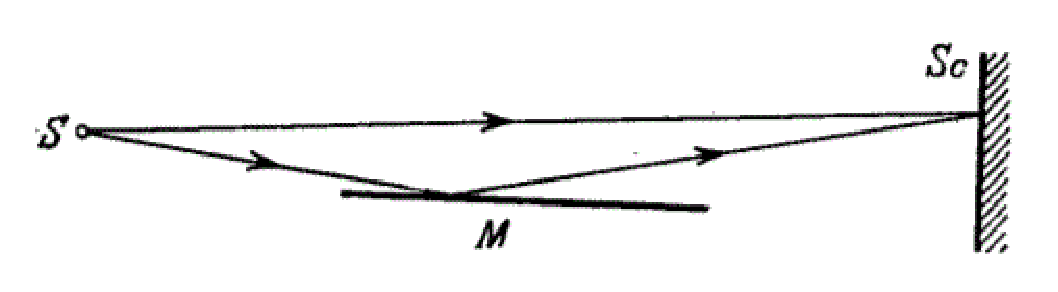
\includegraphics[width=0.5\textwidth]{Pictures/5.69.eps}
\caption{Exercise \ref{5.69}}
\label{fig:5.69}
\end{figure}
\begin{exercise}\label{5.69}
Lloyd의 거울 실험(Figure \ref{fig:5.69})에서, 얇은 슬릿 $S$에서 나온 빛이 거울 M에 반사된 빛과 간섭하여 스크린 Sc에 간섭 무늬가 만들어졌다. 광원은 스크린에서 $l = 100 \mathrm{cm}$만큼 떨어져 있다. 광원이 특정 지점에 있을 때 스크린에 맺힌 간섭 무늬의 폭이 $\Delta x=0.25\mathrm{mm}$였으며, 광원을 거울면에서 $\Delta h =0.60\mathrm{mm}$만큼 멀어지게 했을 때 간섭무늬의 폭은  $\eta = 1.5$배만큼 좁아졌다고 한다. 이때 빛의 파장을 구하여라. (Irodov)
\end{exercise}

\begin{problem}
한쪽 면은 볼록하고 반대쪽 면은 평면인 렌즈(plano-convex lens)가 볼록한 면을 아래로 하여 유리판에 맞닿아있다. 볼록한 면의 곡률이 $R$이고, 빛의 파장은 $\lambda$이라고 한다. 이 때 뉴턴 링 사이의 간격 $\Delta r$을 $r$의 함수로 표현하여라. (단, $\Delta r \ll r$이다.) (Irodov)
\end{problem}

\begin{problem}\label{5.71}
\begin{figure}[h]
\centering
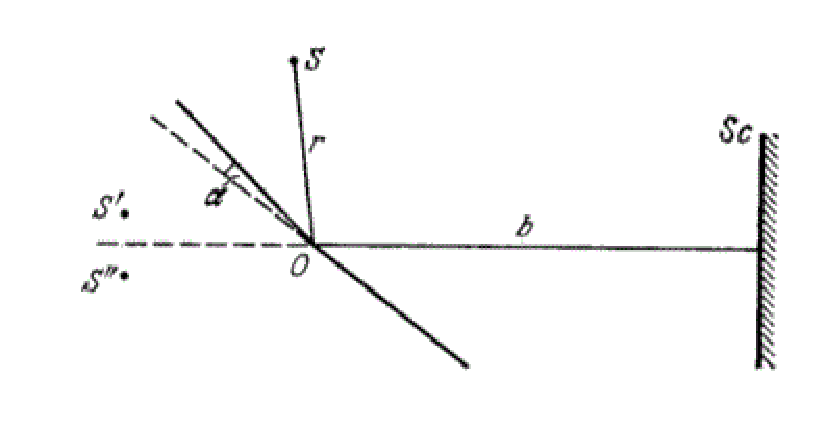
\includegraphics[scale=0.5]{Pictures/5.71.eps}
\caption{Problem \ref{5.71}}
\label{fig:5.71}
\end{figure}
Figure \ref{fig:5.71}은 Fresnel mirrors를 이용한 실험을 나타낸다. 두 거울 사이의 각도 $\alpha = 12'$이고, 두 거울의 교선과 슬릿 $S$, $Sc$까지의 거리는 각각 $r=10.0\mathrm{cm}$, $b=130\mathrm{cm}$이다. 빛의 파장이 $\lambda = 0.55\mathrm{pm}$일 때, (1) 스크린에 맺히는 무늬의 폭을 구하여라. (2) 슬릿이 중심이 $O$이고 반지름이 $r$인 원의 접선 방향으로 $\Delta l=1.00\mathrm{mm}$ 움직였을 때, 간섭 무늬는 얼마나 움직이는가? (3) 스크린에 맺히는 간섭 무늬가 충분히 선명하게 보이기 위한 슬릿의 최대 폭 $\delta_{max}$를 구하여라. (Irodov)
\end{problem}

\begin{problem}
두께 $5.0\mathrm{cm}$, 초점거리가 $f=25.0\mathrm{cm}$인 볼록렌즈를 중심을 따라 이등분하여 사이의 두께 $1.00\mathrm{mm}$인 부분을 깎아낸 후 다시 붙여서 합성 렌즈를 만들었다. Focal plane에 얇은 슬릿이 파장 $\lambda = 0.60\mathrm{\mu m}$의 단색광을 내보내고 있으며 렌즈 뒤쪽으로  $b=50\mathrm{cm}$ 떨어진 지점에 스크린이 놓여 있을 때, (1) 스크린에 맺히는 회절 무늬의 개수와 가능한 maxima의 개수 (2) 회절 무늬가 충분히 선명하게 보이기 위한 슬릿의 최대 두께 $\delta_{max}$를 계산하여라. (Irodov)
\end{problem}

\begin{problem}
Fresnel biprism에게서 $a=25\mathrm{cm}$ 떨어진 곳에 얇은 슬릿이, $b=100\mathrm{cm}$ 떨어진 곳에는 스크린이 위치해 있다. Biprism의 굴절각이 $\theta = 20'$이고 스크린에 맺히는 회절 무늬의 폭이 $\Delta x = 0.55\mathrm{mm}$일 때, 슬릿에서 나오는 빛의 파장을 구하여라. (Irodov)
\end{problem}

\begin{problem}
A microwave transmitter at height $h$ above the horizontal reflective surface(Lloyd's mirror) transmits microwaves of wavelength $\lambda$ toward a receiver on the distance $R$, at the same height $h$ above the mirror. The microwaves reflecting from the mirror interfere with the microwave arriving directly from the transmitter. 
(a) Find an expression that gives the values of R for which the signal at the receiver is maximum. (Hint: Does the reflection cause a phase change?)
(b) If the receiver shows a power $P_0$ at distance from the transmitter without the reflective surface, what is a reading if there is the reflector between them? (2017-2 기출)
\end{problem}


\section{회절}
이번에는 $Nd$를 일정하게 두고 $N\to\infty$로 가는 경우를 생각해보자. 이 경우는 빛이 나오는 곳이 무수히 많기 때문에 슬릿의 두께가 있을 경우의 단일 슬릿 회절무늬와 대응된다. 이 경우 슬릿의 폭은 $w=Nd$라고 할 수 있다.
이때
\begin{align}
I&=I_0 \frac{\sin^2 (k/2\cdot Nd\sin\theta)}{\sin^2 (k/2\cdot d\sin\theta)}\\
&=I_0N^2 \frac{\sin^2 (k/2\cdot w\sin\theta)}{N^2\sin^2 (k/2\cdot d\sin\theta)}\\
&\approx I_0N^2 \frac{\sin^2 (k/2\cdot w\sin\theta)}{N^2\sin^2 (k/2\cdot d\sin\theta)} \frac{\sin^2 (k/2\cdot d\sin\theta)}{(k/2\cdot d\sin\theta)^2}\\
&= I_0N^2 \frac{\sin^2 (k/2\cdot w\sin\theta)}{(k/2\cdot w\sin\theta)^2}
\end{align}
따라서 $\beta = \frac{1}{2}kw\sin\theta$라고 하면 빛의 세기는 
\begin{equation}
I=I_0N^2 \frac{\sin^2 \beta}{\beta^2}
\end{equation}
으로 쓸 수 있다. $N$은 더 이상 의미가 없으므로 $I_0N^2$을 새로 $I_0$로 정의하면, 
\begin{equation}
I=I_0 \frac{\sin^2 \beta}{\beta^2}\label{eq:singlediff}
\end{equation}
이다. 이를 그래프로 나타내면 다음과 같다.
\begin{figure}[h]
\centering\includegraphics[scale=0.5]{Pictures/diffraction.PNG}
\caption{단일 슬릿 회절 무늬}
\label{fig:diffslit}
\end{figure}

원형의 구멈을 통한 회절의 경우, first diffraction minimum을 다음과 같이 얻을 수 있다.
\begin{equation}
\sin\theta=1.22\frac{\lambda}{d}
\end{equation}
이때 $\theta$는 구멍의 중심을 지나는 법선과의 각도를 의미한다. 두 천체를 망원경을 통해 관측할 때와 같은 경우, 렌즈를 통해 바라본 두 천체가 구별되기 위한 기준은 하나의 central maximum이 나머지 하나의 first diffraction minimum 안으로 들어가지 않는 것이다. 이를 레일리 기준(Rayleigh's criterion)이라 한다.

\begin{exercise}
허블 우주 망원경의 주반사경은 지름이 $2.4\mathrm{m}$이다. 이때 초록색 빛에 대한 이 망원경의 angular resolution을 구하여라. (Bauer)
\end{exercise}



\paragraph{회절 격자}
회절 격자(diffraction grating)란 슬릿과 같이 빛을 통과시킬 수 있는 구멍이 수백 개 모여 이루어진 것을 말한다. 또한, 구멍 대신 거울으로 이루어진 회절 격자 또한 존재한다. 회절 격자의 성질로는 분산(dispersion)과 분해능(resolving power)이 있다. 먼저 분산이란 $\lambda$에 따라 회절되는 각도가 얼마나 민감하게 변화하는지 나타내는 척도, 즉 $\theta$의 $\lambda$에 대한 변화율을 말한다. $\sin\theta = m\frac{\lambda}{d}$이므로, 이는
\begin{equation}
D=\frac{d\theta}{d\lambda}=\frac{d}{d\lambda}\left ( \sin^{-1}\left ( \frac{m\lambda}{d}\right )\right)=\frac{1}{\sqrt{1-(\frac{m\lambda}{d})}}\frac{m}{d}=\frac{m}{d\cos\theta}
\end{equation}
로 나타낼 수 있다. \\
해상도란 가까이 있는 두 maxima를 떼어 놓는, 즉 분해하는 능력을 뜻하며 이는 각 maximum의 너비에 의존하는 값이다. 두 maxima의 파장을 각각 $\lambda_1, \lambda_2$라고 할 때, 분해 가능한 파장의 가장 작은 차이가 $\Delta\lambda_{min}=\lambda_2-\lambda_1$이라고 하면, 해상도는
\begin{equation}
R=\frac{\lambda_{avg}}{\Delta \lambda_{min}}
\end{equation}
으로 정의된다. 이때 $\lambda_{avg}=\frac{1}{2}(\lambda_1+\lambda_2)$이다. 그런데 두 광선의 회절 각도를 $\theta_1, \theta_2$라고 할 때, $\Delta \theta = \theta_{hw}$일 때 겨우 분리가 가능하다. 또한 $\theta_{hw}$의 각도는 first diffraction minimum과 같으므로, $\sin\theta_{hw}=\frac{\lambda}{a}=\frac{\lambda}{Nd}$이다. 
\begin{figure}[h]
\centering\includegraphics[scale=0.5]{Pictures/resolving_power.png}
\caption{Central maximum의 half-width}
\label{fig:diffslit}
\end{figure}
$\sin\theta_{hw}\approx \theta_{hw}$이므로 $\theta_{hw} = \frac{\lambda}{Nd}$이며, 일련의 과정을 통해 1차가 아닌 다른 차수의 maxima에서 $\theta_{hw} = \frac{\lambda}{Nd\cos\theta}$임을 보일 수 있다. 그런데 $D=\frac{d\theta}{d\lambda}$이므로 $\Delta\lambda=\frac{\Delta \theta}{D}=\lambda/Nm$이다. 따라서
\begin{equation}
R=\frac{\lambda_{avg}}{\Delta \lambda}=Nm
\end{equation}
임을 알 수 있다.
\paragraph{이중 슬릿 간섭}
이중 슬릿의 경우에는 위의 폭이 있는 단일 슬릿 2개가 $d$의 간격을 두고 중첩되어 있는 것이다. 따라서 식 \ref{eq:singlediff}과  \ref{eq:multslit}을 적용하면 각도 $\theta$에 따른 빛의 세기는 다음과 같이 표현할 수 있다. ($\alpha =\frac{1}{2}\delta = \frac{1}{2}kd\sin\theta$)
\begin{align}
I&=I_0 \frac{\sin^2\beta}{\beta^2}\frac{\sin^2(2\alpha)}{\sin^2(\alpha)}\\
&=4I_0 \frac{\sin^2 \beta}{\beta^2}\cos^2\alpha
\end{align}
파동광학 파트에서는 이상의 유도 과정을 모두 외워두는 것이 좋다.
\begin{exercise}
폭이 $w$인 슬릿 3개가 $d$씩 떨어져 있을 때, 이것이 만들어 내는 무늬를 각도에 따른 세기 형태로 나타내시오.
\end{exercise}

\begin{exercise}
$\lambda=0.50\mathrm{\mu m}$의 파장을 가진 빛이 $b=10\mathrm{\mu m}$의 폭을 가진 슬릿의 법선과 $30^\circ$의 각도를 이루며 입사하고 있다. 이 때 central Fraunhofer maximum의 양 쪽에 형성되는 first minima의 위치를 각도로 표현하여라. (Irodov)
\end{exercise}

\begin{problem}
$\lambda = 530\mathrm{nm}$의 파장을 가진 빛이 $1.50\mathrm{\mu m}$의 주기를 가진 투명한 회절격자로 입사하고 있다. 입사각이 (1) $0^\circ$일 때와 (2) $60^\circ$일 때, 각각 가장 높은 차수의 Fraunhofer maximum의 각도를 구하여라. (Irodov)
\end{problem}

\begin{problem}
Point source 6개가 나란히 있고, lambda = d/2의 파장으로 빛이 나오고 있다. 이때
(1) 1번째 principal maxima의 각도를 구하여라
(2)$-\pi/2\le\theta\le\pi/2$의 범위 안에 있는 principal maxima의 개수를 구하여라.
(3) 첫번째 dark fringe의 각도를 구하여라.
(4) 파장을 바꾸었을 때, 첫번째 principal maximum 바로 옆의 dark fringe였던 자리에 새로운 first principal maximum이 위치하게 된다. 이때 파장을 구하시오. (2019-2 기출)
\end{problem}


\chapter{상대성 이론}
\section{상대성 이론}
\begin{definition}[관성 좌표계]
관성 좌표계(inertial reference frame)란 외부에서 알짜 힘이 작용할 때에만 물체가 가속되는 좌표계를 뜻한다.
\end{definition}
\begin{theorem}[상대성 이론의 가정]
상대성 이론의 기반이 되는 아인슈타인의 가정은 다음과 같다.\\
\begin{enumerate}
\item 물리 법칙은 모든 관성 좌표계에서 같다.
\item 빛의 속도는 모든 관성 좌표계에서 $c=299792458\mathrm{m/s}$로 일정하다.
\end{enumerate}
\end{theorem}
\begin{definition}[$\beta$ 인자와 $\gamma$ 인자]
물체의 속도가 $\vec{v}$일 때, 
\begin{equation}
\vec{\beta}=\vec{v}/c\quad\quad\gamma=\frac{1}{\sqrt{1-\beta^2}}
\end{equation}
로 정의한다. 1차원에서, $-1\le \beta \le 1$이며 $\gamma\ge 1$이다. 
\end{definition}
특수 상대성 이론의 대표적인 두 현상인 길이 수축과 시간 팽창은 물리2에서 이미 배웠을 것이다.

\begin{remark}
정지한 관측자가 측정하였을 때 같은 장소에서 $\Delta t_0$의 간격으로 벌어진 두 사건은, 이 관측자 기준으로 $v$의 속력으로 움직이는 관측자가 측정할 때에는
\begin{equation}
\Delta t = \gamma \Delta t_0=\frac{1}{\sqrt{1-(v/c)^2}}\Delta t_0
\end{equation}
의 간격으로 측정된다.
\end{remark}
\begin{remark}
정지된 관측자가 측정하였을 때 같은 시간에 $\Delta L_0$의 간격으로 벌어진 두 사건은, 이 관측자 기준으로 $v$의 속력으로 움직이는 관측자가 측정할 때에는
\begin{equation}
\Delta L = \Delta L_0 /\gamma = \sqrt{1-(v/c)^2}\Delta L_0
\end{equation}
의 간격으로 측정된다.
\end{remark}

\begin{theorem}[로런츠 변환]
관성계 $S$의 관측자가 보았을 때 시공간 좌표 $(t, x,y,z)$에서 일어난 사건이 $S$에 대해 속도 $\vec{v}=(v,0,0)$의 속도로 움직이는 관성계 $S'$의 관측자가 보았을 때 $(t',x',y',z')$에서 일어났다면, 이는
\begin{equation}
\begin{pmatrix}
ct'\\
x'\\
y'\\
z'\\
\end{pmatrix}
= \begin{pmatrix}
\gamma& -\gamma\beta& 0& 0\\
-\gamma\beta & \gamma & 0 & 0 \\
0&0&1&0\\
0&0&0&1\\
\end{pmatrix}
\begin{pmatrix}
ct\\
x\\
y\\
z\\
\end{pmatrix}
\end{equation}
의 관계를 갖는다. 이를 로런츠 변환(Lorentz transformation)이라고 한다.
\end{theorem}
어떤 두 사건이 $(\Delta t, \Delta x, \Delta y, \Delta z)$만큼의 차이를 두고 일어난다면, $-c^2(\Delta t)^2 +(\Delta x)^2 + (\Delta y ) ^ 2 + (\Delta z)^2$은 어떤 좌표계에서 관측해도 불변이다. 이를 로런츠 불변량(Lorentz invariant)이라고 한다. 이것이 양수라면 두 사건 사이의 간격(interval)이 '공간같다(spacelike)'고 하며, 음수라면 '시간같다(timelike)'고 한다. 0이라면 '빛같다(lightlike)'고 한다.\\
시간같은 간격에 대해
\begin{equation}
-c^2(\Delta t)^2 +(\Delta x)^2 + (\Delta y ) ^ 2 + (\Delta z)^2=-c^2(\Delta \tau)^2
\end{equation}
인 $\Delta \tau$를 고유시간이라고 하며, 공간같은 간격에 대해
\begin{equation}
-c^2(\Delta t)^2 +(\Delta x)^2 + (\Delta y ) ^ 2 + (\Delta z)^2=(\Delta s)^2
\end{equation}
인 $\Delta s$를 고유길이라고 한다. 즉, 고유시간은 두 사건이 같은 장소에서 발생한 것으로 보이는 관측자가 볼 때의 시간 간격이며 고유길이는 두 사건이 같은 시각에 발생한 것으로 보이는 관측자가 볼 때의 길이이다. 만약 두 사건이 원인과 결과의 관계라면 두 사건은 공간같을 수 없다. 공간같다면 $-c^2(\Delta t)^2 +(\Delta x)^2 >0$이므로 $\Delta x/\Delta t>c$가 되기 때문이다. 정보의 전달 속도는 빛보다 빠를 수 없다.
\begin{example}
어떤 관성계에 대해 정지된 관측자가 볼 때, 두 섬광(flash)이 동시에 발생하였다. 이 관측자가 볼 때 두 섬광이 $\Delta x$의 거리를 두고 발생하였다면, 이 관측자에 대해 $0.25c$의 상대속도로 움직이는 다른 관측자가 볼 때에 두 섬광이 일어난 시간의 차이와 거리를 구하여라. 또,  두 사건이 시간같은지, 공간같은지, 또는 빛같은지 말하여라.
\end{example}
먼저, 첫 번째 관측자가 볼 때 두 섬광이 동시에 발생하였다고 하였으므로 두 사건은 '공간같다'라고 할 수 있다. 또한 $\gamma = 4/\sqrt{15}, \beta = 0.25$이므로 
\begin{equation}
\begin{pmatrix}
ct'\\
x'\\
\end{pmatrix}
= \begin{pmatrix}
4/\sqrt{15}& -1/\sqrt{15}\\
-1/\sqrt{15}&4/\sqrt{15}
\end{pmatrix}
\begin{pmatrix}
0\\ 
\Delta x
\end{pmatrix}
= \begin{pmatrix}
-\Delta x/\sqrt{15}\\
4\Delta x/\sqrt{15}\\
\end{pmatrix}
\end{equation}
따라서, 이 관찰자가 보았을 때 두 사건은 $\Delta t'=-\Delta x/\sqrt{15}c$만큼의 시간과 $\Delta x' = 4\Delta x/\sqrt{15}$의 공간을 두고 떨어져 있는 것으로 보인다.

\paragraph{로런츠 속도 변환}
관성계 $S$에서 관측한 속도를 $v$라고 하고, $S$에 대해 $V$의 속도로 운동하는 $S'$에서 관측한 속도를 $v'$이라고 하자. 그러면 $v'=\frac{dx'}{dt'}$이다. 그런데 $\gamma = \frac{1}{\sqrt{1-(V/c)^2}}$라고 할 때, 로런츠 변환에 의해 $dx=\gamma V dt' + \gamma dx'$이고, $dt=\gamma( dt' +\frac{Vdx}{c^2})$이다. 또한, $v=\frac{dx}{dt}$이므로 $dx=vdt$이다. 따라서, 
\begin{equation}
v'=\frac{dx'}{dt'}=\frac{\gamma(V+v)dt}{\gamma(dt+Vvdt/c^2)}=\frac{v+V}{1+vV/c^2}
\end{equation}
임을 알 수 있다. (여러 속도를 더해야 할 때에는 빠르기(rapidity) $\theta = \tanh^{-1}(v/c)$를 정의하면 $\theta'=\Theta +\theta$가 성립하여 편리하다.)

\begin{exercise}
관성계 $S$에서 $v_y$의 속력으로 $+y$ 방향으로 움직이는 물체가 있을 때, $S$에 대해 $+x$ 방향으로 $V$의 속도로 움직이는 관성계 $S'$에 위치한 관측자에게는 이 물체가
\begin{equation}
v_y'=\frac{v_y}{\gamma(1+Vv_y/c^2)}
\end{equation}
로 움직이는 것으로 관측된다. 위와 비슷한 과정을 통해 이를 보여라.
\end{exercise}

\begin{exercise}[등가속도 운동]
어떤 입자가 자신과 함께 움직이는 좌표계를 기준으로 $a$의 가속도로 움직이고 있다. 처음에 이 입자가 정지된 상태에서 출발한다면, 정지된 관측자가 보았을 때 시간이 $t$인 순간에 입자의 속도와 변위를 구하여라. (힌트: 입자의 좌표계는 각 순간에 관성 좌표계로 근사될 수 있다.)
\end{exercise}

\paragraph{상대론적 에너지와 운동량}
$v=\frac{V+v'}{1+v'V/c^2}$일 때, 
\begin{equation}
\gamma_v=\frac{1}{\sqrt{1-(v/c)^2}}=\frac{1+Vv'}{\sqrt{1-(v/c)^2}\sqrt{1-(v'/c)^2}}=\gamma_V\gamma_{v'}(1+Vv')
\end{equation}
임을 보일 수 있다. 따라서
\begin{equation}
v\gamma_v=\gamma_V\gamma_{v'}(V+v')
\end{equation}
이다. 즉, 
\begin{align}
p=\gamma_v mv\quad\quad E=\gamma_v mc^2\\
p'=\gamma_{v'} mv'\quad\quad E'=\gamma_{v'} mc^2
\end{align}
으로 정의하면 
\begin{equation}
p = \gamma_Vm(\gamma_{v'}(V+v'))=\gamma_V (\gamma_v'mc^2/c^2V+p')
\end{equation}
이므로, $\beta = V/c$일 때
\begin{equation}
p=\gamma_V\beta_V (E'/c)+\gamma_Vp'
\end{equation}
이다. 마찬가지로, $(E/c)=\gamma_V (E'/c)+\gamma_V\beta_V p$가 성립한다. 이를 $E'$과 $p'$에 대해 정리하고 $\gamma_V$와 $\beta_V$에서 첨자를 떼면
\begin{equation}
\begin{pmatrix}
E'/c\\
p_x'\\
p_y'\\
p_z'\\
\end{pmatrix}
=\begin{pmatrix}
\gamma& -\gamma\beta& 0& 0\\
-\gamma\beta & \gamma & 0 & 0 \\
0&0&1&0\\
0&0&0&1\\
\end{pmatrix}
\begin{pmatrix}
E/c\\
p_x\\
p_y\\
p_z\\
\end{pmatrix}
\end{equation}
로 쓸 수 있다. 즉, 에너지와 운동량에 대해서도 로런츠 변환이 성립한다. 이에 따라 $(E/c,p_x,p_y,p_z)$를 4-운동량(4-momentum)이라고 한다. 4-운동량에 대해서도 불변량이 존재하는데, 이는 $-(E/c)^2+p_x^2+p_y^2+p_z^2$이다. 이는 어느 관성 좌표계에서 관측하여도 일정하다. 바꾸어 말하면 $E^2-p^2c^2$이 어느 관성 좌표계에서 관측하여도 일정하다고 할 수 있는데, 이를 $v=0$인 좌표계에서 보면 $E=m_0c^2$이므로 $E^2-p^2c^2=m_0c^2$이 항상 성립한다고 할 수 있다.
\begin{theorem}[로런츠 불변량]
두 관성계에서 보았을 때 어떤 입자의 좌표가 각각 $(ct_A, x_A, y_A,z_A)$와 $(ct_B, x_B,y_B, z_B)$이라고 할 때, $-(ct)^2 +x^2 +y^2 +z^2$은 두 관성계에서 동일하다. \\
또한, 마찬가지로 입자의 운동량과 에너지는 어떤 관성계에서 측정되어도
\begin{equation}
E^2 = p^2c^2+(m_0c^2)^2
\end{equation}를 만족시킨다.
\end{theorem}

\\
상대성 이론에서의 충돌 문제는 에너지와 운동량이 항상 모두 보존된다고 가정하고 풀어야 한다. 완전탄성충돌이 아닌 경우에도 입자의 질량이 증가하면서 에너지의 손실이 없게 된다.

\begin{example}
정지질량이 $m_0$이고 운동에너지가 $T$인 입자가 같은 정지질량을 가진 멈춰 있는 입자와 충돌하였다. 두 입자가 합쳐져서 하나의 입자가 되었을 때, 이것의 정지질량과 속도를 구하여라. (Irodov)
\end{example}
어떤 관성계에서 바라보아도 $E^2-p^2c^2$은 일정하다. 첫번째 입자에서, $p_1^2c^2 =E^2-m_0c^2 = (T+m_0c^2)^2-(m_0c^2)^2$이다. 따라서,
\begin{equation}
E^2-p^2c^2=(T+2m_0c^2)^2 -\sqrt{T(T+2m_0c^2)}^2=c^2(2m_0(2m_0c^2+T))
\end{equation}
이다. 그런데, 이는 새로 합쳐진 입자의 관성계에서 보아도 같고, 새 입자의 관성계에서 보면 자신의 속도는 0이므로 이는 $(M_0c^2)^2$과 같다. 따라서 새 입자의 정지질량
\begin{equation}
M_0=\frac{1}{c}\sqrt{2m_0(2m_0c^2+T^2)}
\end{equation}
임을 알 수 있다. 또한, 에너지 보존에 의해 $2m_0c^2+T=\gamma M_0c^2=\frac{M_0c^2}{\sqrt{1-v^2/c^2}}$이 성립하며, 이를 풀면 
\begin{equation}
v=c\sqrt{\frac{T}{T+2m_0c^2}}
\end{equation}
를 얻을 수 있다.(또는 $v=c^2p/E$임을 이용해도 된다)
\begin{exercise}
$E_0$와 $K$가 각각 질량(정지) 에너지와 상대론적 운동에너지일 때, $\beta = \frac{v}{c}=\sqrt{1-(\frac{E_0}{E_0+K})^2}$가 성립함을 보여라.
\end{exercise}

\begin{exercise}
$F=\frac{dp}{dt}=\frac{d}{dt}(\gamma m v)$임을 이용하여 상대론적 운동에너지가 $K=(\gamma -1) mc^2$임을 보여라. 
\end{exercise}


\begin{exercise}
질량이 $m$인 물체가 $v_1=0.8c$의 속도로 멈춰 있는 질량이 $M$인 물체에 충돌하였다. 이후 첫 번째 물체는 반대 방향으로 $v_2=0.6c$의 속도로 튕겨나갔다. 질량 $M$인 물체의 충돌 이후의 속도 $u$를 구하여라. 또, $M$을 $m$으로 나타내어라.
\end{exercise}
상대론에서 충돌 문제를 다룰 때에는 $c=1$으로 두어서 풀면 쉽다. 이후 맨 마지막에 다시 $c$를 여러 번 곱하거나 나누어 단위를 맞추면 된다.

\paragraph{상대론적 도플러 효과}
빛은 매질이 없기 때문에 우리가 알고 있는 도플러 효과가 적용되지 않는다. 대신, 광원과 관측자의 상대속도 $v$에만 의존하는 꼴으로 바뀌게 된다. 광원에서 나오는 빛의 진동수가 $f_0$일 때, 관측자가 측정하는 진동수는
\begin{equation}
f=f_0\sqrt{\frac{c\mp v}{c\pm v}}
\end{equation}
로 표현된다. 또, $c=f\lambda$이므로
\begin{equation}
\lambda=\lambda_0\sqrt{\frac{c\mp v}{c\pm v}}
\end{equation}
또한 성립한다.

\begin{problem}
관성 좌표계 $K$에 위치한 두 불안정한 입자가 일직선상에서 같은 속도 $v=0.990c$로 운동하고 있다. 이 관성계에서 봤을 때 두 입자 사이의 간격은 $l=120\mathrm{m}$이다. 두 입자와 함께 움직이는 관성계에서 봤을 때 두 입자가 동시에 붕괴한다고 하면, $K$에서 봤을 때 두 입자가 붕괴하는 시간 간격은 얼마인가? 또, 어느 입자가 먼저 붕괴하는가? (Irodov)
\end{problem}

\begin{problem}
양 끝점이 각각 $A$와 $B$인 막대가 관성 좌표계 $K$의 $+x$ 방향으로 $v$의 속도를 가지며 움직이고 있다. 이때 $A$는 막대의 앞쪽이며 $B$는 뒷쪽이다. 이때 (a) 특정 시간에 측정했을 때 두 점의 좌표가 $x_A$와 $x_B$라면 막대의 고유길이는 얼마인지 (b) $K$에서 봤을 때 두 좌표값의 차이가 고유길이와 같게 하려면 시간 차이는 얼마가 되어야 하는지 구하여라. (Irodov)
\end{problem}

\begin{problem}
$m_0$의 정지질량을 가진 입자가 정지한 상태에서 3개의 입자로 쪼개진다. 각각의 질량을 $m_1, m_2, m_3$라고 할 때, $m_1$이 가질 수 있는 최대 에너지를 구하여라. (Irodov)
\end{problem}

\begin{problem}
같은 에너지와 같은 질량 $m$을 갖는 전자와 양전자가 $90^\circ$의 각도로 충돌한다. 이것은 충돌 후 쌍소멸하며 질량이 $M$으로 동일한 양성자-반양성자 쌍을 만든다. 생성 이후에 양성자는 움직이지 않는다고 할 때, 처음 전자와 양전자의 에너지를 구하여라. (2019-2 기출)
\end{problem}

\begin{problem}
관찰자 $A$와 우주선 $B, C$가 있다. $v_{B/A}= c/2, v_{C/B}=c/4$이고 세 물체의 초기 위치는 모두 같다. 관찰자 $A$의 시계가 $\tau$ 일 때 $B$에서 $C$ 를 향해 진동수 $f_0$인 빛이 발사된다. 
(1)	빛이 거울 $C$에 반사된 후 다시 $A$로 돌아왔을 때 $A$의 시계가 가리키는 시각을 구하시오
(2)	이 때 $A$가 측정한 $C$의 위치는?
(3)	$A$가 측정한 빛의 진동수는? (2019-2 기출)
\end{problem}


\chapter{양자역학}
\section{양자물리학}
\paragraph{광전효과}
광전효과(photoelectric effect)란 금속에 빛을 비추었을 때 전자가 나오는 현상을 말한다. 이때 광자의 에너지는 $hf$로 표현되는데, $hf=\Phi+K_{max}$의 관계가 성립한다. 이때 $\Phi$는 일함수(work function)으로 금속의 고유한 성질이며, $K_{max}$는 튀어나오는 전자의 최대 운동에너지이다. 이때 모든 전자의 운동에너지가 같지 않은 이유는 맨 바깥쪽 표면에서부터 전자가 튀어나온다면 에너지는 $K_{max}$가 되지만, 그렇지 않는 경우에는 전자가 튀어나오면서 에너지가 손실되기 때문이다. 튀어나온 전자에 전위차를 걸어주면서 전류가 더 이상 측정되지 않는 최소의 전위차인 정지전압(stopping potential) $V_0$를 측정하는 방식으로 $K_{max}$를 측정할 수 있다. 이때 $eV_0=K_{max}$가 성립한다.
\begin{exercise}
$4.00\mathrm{cm^2}$의 면적을 갖는 금속 판에 $300\mathrm{mW/m^2}$의 세기를 갖는 빛이 45도의 각도로 비춰지고 있다. 빛의 파장은 $550\mathrm{nm}$이다. 이때,
(a)	광자의 개수
(b)	광전자가 나오는 효율이 25\%일 때, 흐르는 전류
(c)	일함수가 $2.1\mathrm{eV}$일 때, 전자의 속도
(d)	정지전압을 구하여라. (2019-2 기출)
\end{exercise}

\paragraph{컴프턴 산란}
컴프턴 산란은 빛의 이중성을 보여준 실험이다. 파장 $\lambda$인 빛을 전자에 조사하면 광자가 튕겨나가면서 파장이 길어져 $\lambda'$으로 바뀌게 된다. 이 실험장치를 검출기가 $360^\circ$로 둘러싸게 해두면, $\lambda'$은 빛을 측정하는 각도인 $\theta$와
\begin{equation}
\lambda'-\lambda = \frac{h}{m_ec}(1-\cos\theta)
\end{equation}
의 관계를 가지게 된다. 이때 $m_e=9.109\times10^{-31}\mathrm{kg}$은 전자의 질량이다. 이는 운동량 보존과 에너지 보존으로 식을 세워 유도할 수 있다(교과서 1119페이지).
\begin{exercise}
An X-ray photon with a frequency of $3.3530\times 10^{19}\mathrm{Hz}$ strikes an electron in a metal foil, and the scattered photon is detected at an angle of $32.300°$ relative to the direction of the incoming photon. (1) What are the energies of the incoming and scattered photons, in electron-volts? (2) What is the kinetic energy of the electron after the collision? (3) What is the magnitude of the momentum of the electron after the collision? (Bauer)
\end{exercise}
\paragraph{물질파}
de Broglie는 모든 물질은 파동의 성질을 가지고 있다는 것을 밝혔다. 그 파장은
\begin{equation}
\lambda=\frac{h}{p}
\end{equation}
이며, 이를 드 브로이 파장(de Broglie wavelength)이라고 한다. 상대론에서
\begin{equation}
p=\frac{1}{c}\sqrt{E^2-(m_0c^2)^2}=\frac{1}{c}\sqrt{(K+m_0c^2)-(m_0c^2)^2}=\frac{1}{c}\sqrt{K(K+2m_0c^2)}
\end{equation}
이므로, 이는
\begin{equation}
\lambda=\frac{hc}{\sqrt{K(K+2m_0c^2)}}
\end{equation}
로 표현될 수 있다.

\paragraph{불확정성 원리}
Heisenberg의 불확정성 원리(uncertainty principle)에 의해,
\begin{equation}
\Delta x \Delta p_x \ge \frac{1}{2}\hbar
\end{equation}
이 성립한다. 또한, 에너지와 시간에 대해서
\begin{equation}
\Delta E \Delta t \ge \frac{1}{2}\hbar
\end{equation}
이 성립한다.
\begin{exercise}[수소 원자]
수소 원자의 Bohr 모형에서, $x=R\sin\omega t, p_x=p\cos\omega t$가 성립한다.$\Delta x$와 $\Delta p$를 RMS로 계산할 때, 불확정성 원리로부터 $R\ge \frac{\hbar^2}{mke^2}$이 성립함을 보여라. 이를 보어 반지름이라 한다.
\end{exercise}

\begin{problem}
각각 de Broglie 파장 $\lambda_1, \lambda_2$를 가지는 동일한 입자 2개가 서로 수직으로 움직이고 있다. 이 때 두 입자의 질량 중심에 대한 각 입자의 드 브로이 파장을 구하여라. 
\end{problem}
\section{양자역학}
\paragraph{파동함수}
파동 함수(wave function)란 양자역학적 계의 상태에 관한 정보를 담고 있는 복소 함수로, 일반적으로 $\psi(\vec{r}, t)$로 나타낸다. 파동함수의 절댓값의 제곱 $|\psi|^2=\psi\psi^*$는 그 위치에 입자가 발견될 확률 밀도로 해석되며, 이에 따라
\begin{equation}
\int_{-\infty}^\infty |\psi|^2 dV
\end{equation}
가 항상 성립한다. 파동함수가 $Ae^{i(kx-\omega t)}$ 꼴이라고 가정할 때, 여기에서 운동량과 에너지를 얻어내기 위한 연산자(operator)를 정의할 수 있다. 먼저 운동량 연산자를
\begin{equation}
\hat{p}=-i\hbar \frac{\partial }{\partial x}
\end{equation}
로 정의할 수 있다. 그러면
\begin{equation}
\hat{p}\psi =-i\hbar\cdot ki\psi=\hbar k\psi=\frac{h}{\lambda}=p\psi
\end{equation}
가 성립하게 된다. 또한, 에너지 연산자는
\begin{equation}
\hat{E}=i\hbar \frac{\partial }{\partial t}
\end{equation}
로 정의한다면 
\begin{equation}
\hat{E}\psi = i\hbar (-i\omega)=hf\psi=E\psi
\end{equation}
가 성립하게 된다. 파동함수가 서로 다른 진동수와 파장을 가진 함수들의 중첩인 경우라면, 즉
\begin{equation}
\psi(x,t)=A_1e^{i(k_1x-\omega_1 t)}+A_2e^{i(k_2x-\omega_2t)}+\cdots
\end{equation}
인 경우라면, 입자의 평균 운동량은
\begin{equation}
\int_{-\infty}^\infty \psi^*(x,t) \hat{p_x}\psi(x,t)dx
\end{equation}
로 얻을 수 있다. 마찬가지로 평균 위치와 평균 에너지는
\begin{align}
\int_{-\infty}^\infty \psi^*(x,t) \hat{x}\psi(x,t)dx\\
\int_{-\infty}^\infty \psi^*(x,t) \hat{E}\psi(x,t)dx
\end{align}
로 얻을 수 있다. 이를 양자역학에서의 운동학(kinematics)이라고 할 수 있다.
\paragraph{슈뢰딩거 방정식}
이제 양자역학에서의 역학(dynamics)에 대해 알아보겠다. 뉴턴 역학에서는 $\vec{F}=m\vec{a}$가 역학의 기본이 되는 방정식이었으나, 양자역학에서는 '운동'이라는 개념 자체가 없기 때문에 $\hat{F}=m\hat{a}$와 같은 방식으로는 방정식을 얻을 수 없다. 그러나 에너지를 이용하면 
\begin{equation}
\hat{E}=\hat{KE}+\hat{PE}
\end{equation}
와 같은 식으로 식을 세울 수 있다.
1차원의 경우에 이는  
\begin{equation}
i\hbar\frac{\partial}{\partial x}\psi=\frac{\hat{p}^2}{2m}\psi+\hat{U}\psi
\end{equation}
로 나타낼 수 있다. 그런데 $\hat{U}$는 $\psi$와 관련이 없으므로 $U(x,t)$로 바꿀 수 있고, 
\begin{equation}
\hat{p}^2=(-i\hbar\frac{\partial}{\partial x})^2=-\hbar^2\frac{\partial^2}{\partial x^2}
\end{equation}
이므로 이를 대입하면
\begin{equation}
i\hbar \frac{\partial}{\partial t}\psi(x,t) =-\frac{\hbar^2}{2m}\frac{\partial^2}{\partial x^2}\psi(x,t)+U(x,t)\psi(x,t)
\end{equation}
를 얻을 수 있다. 이를 시간 의존 슈뢰딩거 방정식(time-dependent Schroedinger's equation)이라고 한다. 만약 $U(x,t)$가 시간에 의존하지 않는다면, 다음과 같이 이를 $V(x)$로 쓸 수 있다. 
\begin{equation}
i\hbar \frac{\partial}{\partial t}\psi(x,t) =-\frac{\hbar^2}{2m}\frac{\partial^2}{\partial x^2}\psi(x,t)+V(x)\psi(x,t)
\end{equation}
이 상태에서 $\psi(x,t)=\psi(x)f(t)$로 변수분리(separation of variable)한다. 그러면
\begin{equation}
i\hbar \psi(x) \frac{\partial}{\partial t}f(t) =-\frac{\hbar^2}{2m}f(t)\frac{\partial^2}{\partial x^2}\psi(x)+V(x)\psi(x)f(t)
\end{equation}
가 되고, 양 변을 $\psi(x)f(t)$로 나누면
\begin{equation}
\frac{i}{f(t)} \frac{\partial f(t)}{\partial t} =-\frac{\hbar^2}{2m\psi(x)}\frac{\partial^2 \psi(x)}{\partial x^2}+V(x)
\end{equation}
를 얻을 수 있다. 그런데 좌변과 우변이 각각 $t$와 $x$에만 관련된 함수이므로, 양 변이 같은 상수여야만 한다. 이를 $E$라고 하자. 그러면
\begin{equation}
i\hbar \frac{\partial f(t)}{\partial t}=Ef(t)
\end{equation}
와
\begin{equation}\label{eq:tisch}
-\frac{\hbar^2}{2m}\frac{\partial^2 \psi(x)}{\partial x^2}+V(x)\psi(x)=E\psi(x)
\end{equation}
를 얻을 수 있다. 따라서 $f(t)=e^{-i(E/\hbar)t}$이고, 즉 
\begin{equation}
\psi(x,t)=\psi(x)e^{-i(E/\hbar)t}
\end{equation}
이다. 그런데
\begin{equation}
\hat{E}\psi(x,t)=i\hbar (-iE/\hbar)\psi(x,t)=E\psi(x,t)
\end{equation}
이므로, $E$는 이 계의 에너지임을 알 수 있다. 식 \ref{eq:tisch}를 시간 비의존 슈뢰딩거 방정식(time-independent Schroedinger's equation)이라고 한다. 여기에다 경계($V(x)$가 불연속인 지점)에서의 경계 조건을 적용하면 $\psi(x,t)$를 얻을 수 있다.
\paragraph{무한 퍼텐셜 우물}
\begin{equation}
V(x)=\begin{cases}
0\quad 0\leq x \leq a \\
\infty\quad \mathrm{otherwise}\\
\end{cases}
\end{equation}
로 주어진 경우를 무한 퍼텐셜 우물(infinite potential well)이라고 한다. 이 경우 $x<0, a<x$일 대에는 $V(x)$가 무한하므로 $V(x)\psi(x)$가 유한하려면 $\psi(x)=0$이어야만 한다. $0\leq x\leq a$일 때는
\begin{equation}
-\frac{\hbar^2}{2m}\frac{\partial^2 \psi}{\partial x^2}=E\psi(x)
\end{equation}
이므로 해는 삼각함수이며, $\psi(0)=0, \psi(a)=0$임을 생각하면 해는 사인함수이고, $\psi(x)=A\sin(kx)$이고 $k=\sqrt{\frac{2mE}{\hbar^2}}$으로 둘 때 $ka=n\pi$가 성립해야 한다. 이때 $n=0,1,2,\cdots$이고, $n=0$일 때는 정규화할 수 없으므로 $n=1,2,3,\cdots$이다. 
$\int_{-\infty}^\infty \psi\psi^*dx=1$으로 정규화하면 $A=\sqrt{a/2}$이다. 즉,
\begin{equation}
\psi(x) = \sqrt{\frac{a}{2}}\sin(\frac{n\pi x}{a})
\end{equation}
이다. 또한 $k=\sqrt{\frac{2mE}{\hbar^2}}$에서,
\begin{equation}
\frac{n\pi}{a}\hbar=\sqrt{2mE_n}
\end{equation}
이고, 
\begin{equation}
E_n = \frac{n^2h^2}{8ma}
\end{equation}
가 성립한다. 즉, 에너지가 양자화되어 있는 것을 알 수 있다. 
\paragraph{2차원 무한 퍼텐셜 우물}
이번에는 
\begin{equation}
V(x,y)=\begin{cases}
0\quad 0\le x\le a \;\mathrm{and}\; 0\le y\le b\\
\infty\quad \mathrm{otherwise}\\
\end{cases}
\end{equation}
인 경우를 생각하자. 이 경우 에너지가 0인 곳에서
\begin{equation}
-\frac{\hbar^2}{2m}\left (\frac{\partial^2}{\partial x^2}+\frac{\partial^2}{\partial y^2}\right)\psi(x,y)=E\psi(x,y)
\end{equation}
가 성립한다. $\psi(x,y)=g(x)h(y)$로 변수분리한 후 양 변을 $g(x)h(y)$로 나누면
\begin{equation}
-\frac{\hbar^2}{2m}\left \{ \frac{g''(x)}{g(x)}+\frac{h''(y)}{h(y)}\right\}=E
\end{equation}
가 성립한다. 따라서 $x$에 대한 항과 $y$에 대한 항이 각각 일정해야 하고, 이를 $E_x, E_y$라고 할 수 있다($E=E_x+E_y$). 그러면
\begin{align}
-\frac{\hbar^2}{2m}\frac{d^2 g}{d x^2}=E_xg(x)\\
-\frac{\hbar^2}{2m}\frac{d^2 h}{d y^2}=E_yh(y)\\
\end{align}
를 얻을 수 있고, 1차원 무한 퍼텐셜 우물에서와 마찬가지로 풀 수 있다. 그러면 
\begin{equation}
E_x=\frac{h^2n^2}{8ma^2},\quad E_y=\frac{h^2m^2}{8mb^2}\\
\end{equation}
이며, 에너지는 이 둘의 합이다.

\begin{exercise}
세 변의 길이가 모두 $a$인 3차원 무한 퍼텐셜 우물에 대해서 바닥상태와 첫 번째에서 다섯 번째 들뜬상태까지의 에너지를 구하여라. 
\end{exercise}

\begin{exercise}
1차원 무한 퍼텐셜 우물의 파동함수가 모두 서로 정규직교(orthonormal)임을 보여라. 즉, 
\begin{equation}
\int_0^a \psi_n(x)\psi_m(x) dx = \delta_{nm}
\end{equation}
임을 보여라. (단, $\delta_{nm}$은 $n=m$일 때 1, $n\ne m$일 때 0이다.)
\end{exercise}

\paragraph{반유한 퍼텐셜 우물}
반유한 퍼텐셜 우물(Half-finite potential well)은 퍼텐셜 에너지가
\begin{equation}
V(x)=\begin{cases}
\infty\quad x<0\\
0\quad 0\leq x \leq a\\
U_0 \quad x>a\\
\end{cases}
\end{equation}
인 경우를 말한다. 이는 계의 에너지 $E$가 $U_0$보다 작은 경우와 큰 경우로 나눌 수 있다. $E<U_0$인 경우에 고전적으로는 전자가 $x>a$에 존재할 수 없겠지만, 양자역학에서는 $x>a$에서도 존재할 확률이 있다.
\begin{enumerate}
\item $E>U_0$인 경우\\
먼저 $x<0$인 구간에서는 $\psi(x)=0$이다.\\
$0\le x \le a$에서, \begin{equation}
-\frac{\hbar^2}{2m}\frac{d^2\psi}{dx^2}=E\psi
\end{equation}
이므로 $\psi(x)=A\sin(kx)$일 때, $k=\sqrt{\frac{2mE}{\hbar^2}}$에 대해 $ka=n\pi$이다.\\
$x>a$에서는 
\begin{equation}
-\frac{\hbar^2}{2m}\frac{d^2\psi}{dx^2}=(E-U_0)\psi
\end{equation}
이므로 $k'=\sqrt{\frac{2m(E-U_0)}{\hbar^2}}$일 때 $\psi(x) = C\sin(k'x+\phi)$ 꼴이 된다. 경계에서 $\psi$가 연속이 되어야 한다는 조건만으로는 조건이 충분하지 않으므로, 경계에서 $\psi'$이 연속이 된다는 조건까지 추가하여야 한다. 그러면
\begin{align}
A\sin ka&=C\sin(k'a+\phi)\\
Ak\cos ka &= Ck'\cos(k'a+\phi)
\end{align}
이다. 즉 문자는 3개인데 조건은 2개밖에 없으므로 이를 풀 수 없다. $\int_{-\infty}^\infty |\psi(x)|^2 dx=1$임을 이용하면 풀 수 있다고 생각할 수도 있으나 travelling wave에서는 이러한 조건을 사용할 수 없다. 즉, 에너지는 양자화되지 않는다

\item $E<U_0$인 경우
$x<0$에서와 $0\le x \le a$에서는 위의 경우와 같이 각각 $\psi(x)=0$과 $\psi(x)=A\sin(kx)$의 해를 갖는다.\\
반면, $a<x$에서는
\begin{equation}
\frac{\hbar^2}{2m}\frac{d^2\psi}{dx^2}=(U_0-E)\psi
\end{equation}
에서 $U_0-E>0$이므로해는
\begin{equation}
    \psi(x)=Be^{-\gamma x},\; \gamma = \sqrt{\frac{2m(U_0-E)}{\hbar^2}}
\end{equation}
의 꼴이다. $e^{\gamma x}$도 가능하긴 하지만 이 경우 $\psi$가 $x\to \infty$에서 발산하게 된다. 경계조건을 적용하면
\begin{align}
    A\sin ka &= Be^{-\gamma a}\label{eq:bc1}\\
    Ak\cos ka &= -B\gamma e^{-\gamma a}\label{eq:bc2}
\end{align}
를 얻는다. $ka=\alpha, \gamma a=\beta$로 치환한 후,
(\ref{eq:bc1})/(\ref{eq:bc2})를 하고 양 변를 $a$로 나누면
\begin{equation}
    \frac{\tan\alpha}{\alpha}=-\frac{1}{\beta}\label{eq:bc3}
\end{equation}
를 얻을 수 있고, 
\begin{equation}
    \alpha^2+\beta^2 = c =\frac{2mU_0a^2}{\hbar^2}\label{eq:bc4}
\end{equation}
이다. 이 두 식을 연립하면 된다. 이를 그래프로 그려보면 식 \ref{eq:bc3}은 $\beta=-\alpha\cot \alpha$와 같고, 식 \ref{eq:bc4}은 원의 방정식이므로 다음과 같은 그래프를 얻을 수 있다.
\begin{figure}[h!]
\centering\includegraphics[scale=0.4]{Pictures/semiinfinite.PNG}
\caption{반유한 퍼텐셜 우물}
\label{fig:half-finite}
%\addcontentsline{toc}{figure}{Figure \ref{fig:placeholder}} % Uncomment to add the figure to the table of contents
\end{figure}
이때 교점이 나타내는 것이 바로 가능한 $(\alpha, \beta)=(ka,\gamma a)$의 쌍이다. 즉 $c =\frac{2mU_0a^2}{\hbar^2}$의 값에 따라서 가능한 상태의 수가 결정된다. 또한, $\sqrt{c}<\frac{\pi}{2}$이면 해가 없으므로 바닥 상태가 존재하기 위해서는  $U_0>\frac{\hbar^2\pi^2}{8ma^2}$여야만 한다는 것을 알 수 있다.
\end{enumerate}

\paragraph{유한 퍼텐셜 장벽}
\begin{equation}
V(x)=\begin{cases}
\infty\quad x<0\\
0\quad 0\le x\le a\\
U_1 \quad a< x\le b\\
0 \quad x>b\\
\end{cases}
\end{equation}
와 같이 퍼텐셜이 주어졌을 때를 유한 퍼텐셜 장벽(finite potential barrier)이라고 한다. 고전적으로는 $E<U_1$일 경우 입자가 $x>b$에서 존재할 수 없으나 양자역학에서는 존재할 확률이 있다. 이를 터널링(tunneling) 현상이라고 한다.

\begin{figure}[h!]
\centering\includegraphics[scale=0.4]{Pictures/tunneling.PNG}
\caption{유한 퍼텐셜 장벽에서의 터널링}
\label{fig:tunneling}
%\addcontentsline{toc}{figure}{Figure \ref{fig:placeholder}} % Uncomment to add the figure to the table of contents
\end{figure}
$E<U_1$의 경우, 슈뢰딩거 방정식을 풀면 $0\le x\le a, b<x$에서는 삼각함수 꼴의 파동함수가 나오게 되고 $a< x\le b$에서는 $Ce^{-\gamma x}$ 형태의 파동함수가 나온다.  이때 경계 조건을 사용하여 파동함수를 얻을 수 있다. 터널링이 일어날 때의 투과 계수는
\begin{equation}
T=\frac{|\psi(b)|^2}{|\psi(a)|^2}=e^{-2\gamma(b-a)}
\end{equation}
로 정의된다.

\begin{problem}
슈뢰딩거 방정식을 이용해서 퍼텐셜 에너지 $U(x)$에 유한 개의 불연속점이 있더라도 $\psi'(x)$는 연속임을 보여라. (Irodov)
\end{problem}

\begin{problem}
퍼텐셜 에너지가
\begin{equation}
U(x)=\begin{cases}
0\quad x<0\\
U_0\quad x\ge 0
\end{cases}
\end{equation}
로 주어질 때, $m$의 질량과 $E$의 에너지를 가진 입자가 존재한다. 이때 (1) $E>U_0$일 때의 반사 계수(reflection coefficient) $R$을 구하여라. (2) $E<U_0$일 때, 입자의 유효 투과깊이(effective penetration depth)를 구하여라. 즉, 확률밀도함수가 $1/e$이 되는 깊이를 구하여라. (Irodov)
\end{problem}

\begin{problem}
세 변의 길이가 각각 $a, 2a, 3a$인 3차원 무한 퍼텐셜 우물에 전자가 있다. 이때, (1) 바닥 상태의 파동함수 (2) 바닥 상태의 에너지 (3) 첫 번째 들뜬 상태에서 세 번째 들뜬 상태로 전이될 때의 에너지 차 (4) 이 상태에서 다시 바닥 상태로 떨어질 때, 가능한 파장의 개수 (5) (4)의 파장 중 가장 짧은 파장을 구하여라. (2019-2 기출)
\end{problem}

\begin{problem}[조화 진동자]
양자수를 모르는 조화 진동자의 파동함수가 
\begin{equation}
\psi(x) = \left (\frac{\alpha}{\pi}\right ) ^ {1/4} \frac{1}{\sqrt{2}}(2\alpha x^2 -1)e^{-\alpha x^2 /2}
\end{equation}
로 주어져 있다고 한다. 퍼텐셜 에너지가 $V(x) = \kappa x^2 /2$일 때, (1) 파동함수를 시간 비의존 슈뢰딩거 방정식에 대입하여 $\alpha$와 $\kappa$ 사이의 관계를 알아내어라. (2) $\omega=\sqrt{\kappa /m}$일 때, 조화 진동자의 에너지는 $E_n = (n+1/2)\hbar\omega$이다. 이를 통해 주어진 파동함수의 양자수 $n$을 구하여라.
\end{problem}

\section{수소원자의 보어 모형}
보어 모형은 닐스 보어에 의해 제안된 원자 모형으로, 원자핵 주변을 도는 전자의 각운동량이 양자화되어 있다는 가정을 기반으로 한다. 
\begin{equation}
|\vec{L}|=|\vec{r}\times \vec{p}|=r\mu v=n\hbar
\end{equation}
이를 양자 조건이라고 한다. 이때 $\mu=\frac{mM}{m+M}$으로, 원자핵과 전자의 환산질량이다. 원자핵의 질량이 전자에 비해 훨씬 크기 때문에 이는 전자의 질량과 거의 같다. $p=\mu v=\frac{h}{\lambda}$이므로 이는
\begin{equation}
\lambda = \frac{2\pi r}{n}
\end{equation}
로 바꿔쓸 수 있다. 또한, 뉴턴 제2법칙에 의해
\begin{equation}\label{eq:N2}
\frac{\mu v^2}{r}=\frac{1}{4\pi \epsilon_0}\frac{e^2}{r^2}
\end{equation}
가 성립한다. 첫 번째 식에서 $v=\frac{n\hbar}{r\mu}$를 식 \ref{eq:N2}에 대입하면 
\begin{equation}
\frac{\mu}{r}\left(\frac{n\hbar}{r\mu}\right)^2=\frac{e^2}{4\pi\epsilon_0r^2}
\end{equation}
이므로
\begin{equation}
r_n=\frac{4\pi \epsilon_0 n^2\hbar^2}{\mu e^2}
\end{equation}
가 성립한다. 바닥 상태($n=1$)일 때 이를 수소 원자의 보어 반지름(Bohr's radius)이라 하며, $a_0$로 쓴다. 또한 각 양자수에서의 에너지는 
\begin{equation}
E_n=KE+PE=\frac{1}{4\pi \epsilon_0}\frac{e^2}{2r_n}-\frac{1}{4\pi \epsilon_0}\frac{e^2}{r_n}=-\frac{1}{4\pi \epsilon_0}\frac{e^2}{2r_n}
\end{equation}
이므로,
\begin{equation}
E_n=-\frac{\mu e^4}{32\pi^2\epsilon_0^2n^2\hbar^2}= -\frac{2.18\times 10^{-18}}{n^2}\mathrm{J}=-\frac{13.6}{n^2}\mathrm{eV}
\end{equation}
이 성립한다. 상태간의 전이가 일어날 때에는 에너지 차이만큼에 해당하는 빛을 방출하거나 흡수하게 된다.
\begin{example}
$m$의 질량을 가진 입자가 $U(r)=kr^2/2$의 구대칭 퍼텐셜 장에서 원운동하고 있다. 보어의 양자 조건을 이용하여 가능한 반지름과 에너지 준위를 구하여라. (Irodov)
\end{example}
주어지는 에너지의 형태가 다르지만 Bohr 모형과 마찬가지의 조건들을 사용하여 풀 수 있다. 먼저 각운동량은
\begin{equation}
|\vec{L}|=mrv=n\hbar
\end{equation}
이고, 구심력은 크기가 $F=-dU/dr=-kr$이므로 
\begin{equation}
m\frac{v^2}{r}=kr
\end{equation}
이 성립한다. 이 두 식을 연립하면
\begin{equation}
r=\left ( \frac{n^2\hbar^2}{km}\right )^{1/4}\quad\quad E_n = \frac{1}{2}kr^2 + \frac{1}{2}mv^2 = mv^2 = kr^2 = \sqrt{\frac{n^2\hbar^2}{km}}k=n\hbar \sqrt{\frac{k}{m}}
\end{equation}
를 얻을 수 있다.
\begin{exercise}[환산질량 보정]
원자핵과 전자가 각각 둘의 질량중심을 기준으로 운동하면 위의 유도과정과 같이 환산질량 $\mu$를 사용하는 것 같은 결과가 나온다는 것을 보여라.
\end{exercise}

\begin{problem}
첫 번째 Bohr 궤도를 돌고 있는 전자에 의해 원자의 중심에서 유도되는 자기장의 크기를 구하여라. (Irodov)
\end{problem}

\begin{problem}
고전 전자기학에 의하면 $a$의 가속도로 움직이는 전자는 전자기파 방사에 의해
\begin{equation}
\frac{dE}{dt}=-\frac{\mu_0c^6}{6\pi c}a^2
\end{equation}
의 속도로 에너지를 잃게 된다. 전자의 각속도가 $5.0\cdot 10^{15}\mathrm{s^{-1}}$일 때, 전자의 에너지가 10배 줄어들기까지 걸리는 시간을 구하여라. (Irodov) 
\end{problem}

\begin{problem}
수소 원자와 $\mathrm{He^+}$ 이온에 대해서,
(1) 첫 번째 보어 궤도의 반지름과 전자의 속도 (2) 바닥 상태에 있는 전자의 운동 에너지와 결합 에너지 (3) 이온화 에너지와 first excitation potential, $n=2\to n=1$로 갈 때 방출하는 빛의 파장을 구하여라. (Irodov)\end{problem}

\begin{problem}
Hydrogen-like system에서 $n$번째 궤도의 운동에 대한 자기 모멘트를 계산하고, 자기 모멘트와 각운동량의 비 $\mu_n/L_n$을 계산하여라. (Irodov)
\end{problem}

\begin{problem}
수소 원자가 정지해 있는 다른 수소 원자와 비탄성 충돌을 하여 정지해 있던 원자가 광자를 내놓았다. 이때 첫 번째 수소 원자의 최소 운동에너지를 구하여라.(단, 두 원자는 충돌 이전에 모두 바닥 상태에 있었다고 가정한다.) (Irodov)
\end{problem}

\begin{problem}
$+Ze$의 전하를 가진 핵 주위로 두 개의 전자가 Bohr-like orbit을 따르며 같은 반지름 $r$으로 돌고 있다고 한다. 두 전자는 항상 핵을 기준으로 원자의 정반대 편에 위치한다. (1) 각 전하에 핵 방향으로 작용하는 알짜힘이 $F=\frac{e^2}{4\pi \epsilon_0 r^2}(Z-\frac{1}{4})$임을 보여라. (2) 보어의 각운동량 조건을 이 원자에 적용하여, $L=\hbar$이라면 이 원자의 반지름이 $r=\frac{\epsilon_0 h^2 }{\pi m e^2 (Z-1/4)}$가 됨을 보여라. (3) 이 원자의 총 에너지를 계산하여라.
\end{problem}


